\documentclass{article}
\usepackage[noend]{algorithmic}
\usepackage{hyperref}
\usepackage{mathtools}

\title{Proyecto ADA, primer entregable}
\author{Jean Miraval y  Mateo Noel}


\newcommand{\TITLE}[1]{\item[#1]}
\renewcommand{\algorithmiccomment}[1]{$/\!/$ \parbox[t]{4.5cm}{\raggedright #1}}
\newbox\fixbox
\renewcommand{\algorithmicdo}{\setbox\fixbox\hbox{\ {} }\hskip-\wd\fixbox}
\renewcommand{\algorithmicthen}{\setbox\fixbox\hbox{\ {} }\hskip-\wd\fixbox}
\newcommand{\algcost}[2]{\strut\hfill\makebox[1.5cm][l]{#1}\makebox[4cm][l]{#2}}


\begin{document}
	\maketitle
	\section{Introducción}
	Para poder resolver el problema de Min-Matching con el uso de estos algoritmos primero decidimos convertir las cadenas de 0's y 1's en vectores de enteros.\\\\
	Por ejemplo: \\Una cadena A=[00111001], será representada como un vector  A = \{3,1\}. \\\\
	Esto es posible gracias a una función getBlocks: \\\\
	Recibe:
	\begin{itemize}
		\item Vector A en binario (bool)
	\end{itemize}
	Devuelve: 
	\begin{itemize}
		\item Vector A en pesos (int)
	\end{itemize}
	\begin{algorithmic}[1]
		\TITLE{\textsc{getBlocks}$(A)$}
		\STATE vector $<$int$>$ blocks
		\FOR {$i=0$ TO A.size() }
		\IF {A[i]}
		\WHILE {A[i]}
		\STATE	newBlock++
		\STATE i++
		\ENDWHILE
		\STATE blocks.push\_back(newBlock);
		\ENDIF
		\STATE return blocks
		\ENDFOR
	\end{algorithmic}
	-\\
	Nota: El código igual recibe como input el tamaño de las cadenas, p, y estas mismas. Solo que las transformará a esta forma de representación.
	
	\section{Secuencias} 
	\subsection*{Pregunta 1 (Voraz)} 
	Para el diseño de un algoritmo voraz, se partió desde la intención de elegir las conexiones analizando únicamente la situación actual, es decir en qué bloque de A o B estamos iterando. El objetivo del algoritmo es hallar el matching correcto entre los dos arrays que tenga el peso mínimo. Como se puede ver desde las fórmulas dadas, el peso de un Matching depende de una suma de pesos de diferentes conexiones. Entonces la estrategia voraz analizada deberá de buscar la manera de formar conexiones con el menor peso posible.
	\\\\Estrategia: Armar conexiones minimizando el peso de estas.
	\\\\Observando las fórmulas, podemos concluir que para minimizar el peso de estas, deberíamos procurar que la suma de los pesos de los bloques de B debe de ser mayor que las de A en cada conexión, para así minimizar el peso que resultará de la división. En base a esto, planteamos nuestra estrategia específica, la cual se basa en formar conexiones buscando dentro de lo posible que la suma de los bloques de A sea menos a la suma de los bloques de B.\\\\ Estrategia: Armar conexiones donde la suma de bloques de B sea mayor que las de A.\\\\
	A partir de este análisis planteamos un pseudocódigo basado en analizar, a medida que avanzamos por una de las listas, si en todo momento la suma de los pesos de A y B permiten seguir haciendo conexiones de tal manera que cumpla con la estrategia. En caso contrario, se aplicaría un Reset Connection, que terminaría esa conexión e iniciaría una nueva a partir de los siguientes bloques. Se añadió las condiciones de combined y divided para evitar interferir con la condición del problema, donde un bloque de A no puede ser agrupado y dividido a la vez.
	
	Recibe: 
	\begin{itemize}
		\item Vectores A y B
	\end{itemize}
	Devuelve: 
	\begin{itemize}
		\item Peso Min-Matching tipo Float
	\end{itemize}
	\begin{algorithmic}[1]
		\TITLE{\textsc{Min-Matching-Voraz}$(A, B)$}
		\algcost{\textit{cost}}{\textit{times}}
		\STATE Divided=0 \algcost{$.$}{$.$}
		\STATE Combined=0 \algcost{$.$}{$.$}
		\STATE Peso=0 \algcost{$.$}{$.$} 
		\STATE BCurrentw = w(B1) \algcost{$.$}{$.$} 
		\STATE ACurrentw = w(A1) \algcost{$.$}{$.$} 
		\STATE Conectar(1,1) \algcost{$.$}{$.$} 
		\STATE BCurrent = 1 \algcost{$.$}{$.$} 
		\STATE ACurrent = 1\algcost{$.$}{$.$} 
		\FOR{$i=2$ TO max(sizeA,sizeB)}  
		\IF {BCurrent $<$ sizeB and ACurrent $<$ sizeA}
		\IF {ACurrentW $<$ BCurrentW}
		\IF {ACurrent $<$ sizeA-1}
		\IF {Divided or Acurrentw + w(Ai) $>=$ Bcurrentw}
		\STATE \textsc{reset-conection}$(...)$ 
		\ELSE 
		\STATE conectar(i,BCurrent)
		\STATE	ACurrentw = ACurrentw + w(Ai)
		\STATE	ACurrent = i
		\STATE	combined = 1
		\STATE	divided = 0
		\ENDIF
		\ELSE 
		\STATE \textsc{reset-conection}$(...)$ 
		\ENDIF
		\ELSE
		\IF {ACurrent $<$ sizeA-1}
		\IF {if combined or BCurrent $>=$ sizeB-1}
		\STATE \textsc{reset-conection}$(...)$ 
		\ELSE 
		\STATE BCurrent++
		\STATE i--
		\STATE conectar(A[ACurrent], B[BCurrent])
		\STATE divided =1
		\STATE combined=0
		\ENDIF
		\ELSE
		\STATE  \textsc{reset-conection}$(...)$ 
		\ENDIF
		\ELSIF{BCurrent ==sizeB}
		\STATE ACurrent++
		\STATE conectar(A[ACurrent], B[BCurrent])
		\ELSE 
			\STATE BCurrent++;
			\STATE conectar(A[ACurrent], B[BCurrent]);
		\IF {BCurrent == sizeB-1} 
		\STATE break
		\ENDIF
		\ENDIF
		\ENDIF
		\ENDFOR
		\STATE peso += ACurrentw/BCurrentw
		\STATE return peso
	\end{algorithmic}
-----------\\
	\begin{algorithmic}[1] 
	\TITLE{\textsc{Reset-conection}$( ... )$}
	\STATE BCurrent++
	\STATE ACurrent++
	\STATE peso += ACurrentw / BCurrentw 
	\STATE conectar(ACurrent, BCurrent)
	\STATE ACurrentw = w(ACurrent) 
	\STATE BCurrentw = w(BCurrent)
	\end{algorithmic}

-----------\\\\
	\textbf{Análisis de Tiempo}\\
	Como podemos observar en el código, la mayoría de las instrucciones dependen de un costo constante y se repetiría las veces que se ejecute la línea del bucle.\\Este bucle itera el máximo entre el array de bloques de A de tamaño m y  array de bloques de B de tamaño n. Todo el código dependerá del max(m,n)\\
	
	$T(m,n) = O(max\{m,n\})$
	

	\subsection*{Pregunta 2 (Recurrencia)}
	Para plantear el problema con recursividad, y con los conocimientos que se obtuvo al realizar el primer problema, nos dimos cuenta de que el solo añadir un bloque diferente, podría ocasionar en ciertos casos la reestructuración de todas las conexiones realizadas previamente. Por este motivo, no era posible realizar una recurrencia donde el resultado de OPT(i,j) esté relacionado directamente con una respuesta anterior. Por lo tanto, para el diseño de la recurrencia, se tomó en cuenta el uso de la recurrencia únicamente para mapear todas las combinaciones posibles del problema partiendo desde los casos iniciales, para posteriormente comparar cada una de ellas y elegir la más óptima, es decir para el problema. Por razones obvias, esta recurrencia es muy costosa en cuanto a recursos y tiempo.
	\\\\
	Donde m = A.size y n = B.size
	\begin{equation*}
	OPT(i,j) =
	\begin{cases}
	A_i / \sum_{x=j}^{n-1}B_x & i = m-1\\\\
	\sum_{x=i}^{m-1}A_x / B_j & j = n-1\\\\
	min(\\
	min_{w=i}^{m-2}( \sum_{x=i}^{w}A_x/ B_j + OPT(w+1, j+1))\\
	min_{w=j+1}^{n-2}(A_i/\sum_{x=j}^{w}B_x + OPT(i+1,w+1))\\
	) & \text{caso contrário}
	\end{cases}
	\end{equation*}
	\subsection*{Pregunta 3 (Recursivo) }
	Utilizando la recursividad planteada en la pregunta anterior, se pasó a ejecutar un algoritmo recursivo, donde utilizamos la recurrencia planteada para elegir el caso más óptimo para cada combinación de bloques de longitud m y n posibles con los inputs dados.\\\\
	Recibe:
	\begin{itemize}
		\item a = donde iniciará A
		\item b = donde iniciará B
		\item vector A y B
	\end{itemize}
	Devuelve: 
	\begin{itemize}
		\item Peso Min-Matching tipo Float
	\end{itemize}
	\begin{algorithmic}[1]
		\TITLE{\textsc{Min-Matching-Recursivo}$(A, B, a, b)$}
		\algcost{\textit{cost}}{\textit{times}}
		\IF{a = m-1  \algcost{$.$}{$.$}}  
		\STATE return $A_a / \sum_{x=b}^{n-1}B_x$ \algcost{$.$}{$.$}
		\ENDIF 
		\IF{b = n-1 \algcost{$.$}{$.$}} 
		\STATE return $\sum_{x=a}^{m}A_x / B_b$ \algcost{$.$}{$.$}
		\ENDIF 
		\STATE vector$<$int$>$ posibles \algcost{$.$}{$.$}
		\FOR{$i=a$ TO $m-2$ \algcost{$.$}{$.$}}
		\STATE p = $\sum_{x=a}^{i}A_x/ B_b + $ \\
		$\text{Min-Match-Rec}(A, B, i+1, b+1)$ \algcost{$.$}{$.$}
		\STATE posibles.push\_back(p) \algcost{$.$}{$.$}
		\ENDFOR
		\FOR{$i=b$ TO $n-2$ \algcost{$.$}{$.$}}
		\STATE p = $A_a / \sum_{x=b}^{i}B_x + $ \\
		$\text{Min-Match-Rec}(A, B, a+1, i+1)$ \algcost{$.$}{$.$}
		\STATE posibles.push\_back(p) \algcost{$.$}{$.$}
		\ENDFOR
		\STATE return min(posibles)  \algcost{$.$}{$.$}
	\end{algorithmic}

-----------\\\\
\textbf{Análisis de Tiempo}\\
Por cada iteración  se resolverán todos los subproblemas, entonces:\\

$T(m,n) = \Omega(2^{max\{m,n\}})$

	\subsection*{Pregunta 4 (Memoizado)}
	Partiendo desde el código anterior, se le añadirá únicamente el cambio de consulta de memoria del algoritmo, implementada a modo de una matriz. Antes de entrar a cálculos de la recursividad compleja, se consultará si el resultado ya ha sido calculado previamente. Además, en caso se ejecute con una combinación de parámetros que aún no ha sido calculada como solución, se almacenará esta solución a la matriz de memoria. De esta forma, luego de las ejecuciones iniciales, cualquier ejecución del algoritmo con una combinación de parámetros ya calculada, tendrá un tiempo de ejecución constante.
	\\\\
		Recibe:
		\begin{itemize}
			\item a y b, índice de inicio dentro del  subproblema en A y B
			\item Vector A y B
			\item M[m][n] donde se guardarán subproblemas
		\end{itemize}
		Devuelve: 
		\begin{itemize}
		\item Peso Min-Matching tipo Float
		\end{itemize}
	\begin{algorithmic}[1]
		\TITLE{\textsc{Min-Matching-Memoizado}$(A, B, a, b, M)$}
		\algcost{\textit{cost}}{\textit{times}}
		\IF{M[a][b] 	\algcost{$.$}{$.$}}
		\STATE return M[a][b]	\algcost{$.$}{$.$}
		\ENDIF
		\IF{a = m-1  \algcost{$.$}{$.$}}  
		\STATE M[a][b] $= A_a / \sum_{x=b}^{n-1}B_x$ \algcost{$.$}{$.$}
		\STATE return M[a][b] \algcost{$.$}{$.$}
		\ENDIF 
		\IF{b = n-1 \algcost{$.$}{$.$}} 
		\STATE M[a][b] $= \sum_{x=a}^{m}A_x / B_b$ \algcost{$.$}{$.$}
		\STATE return M[a][b] \algcost{$.$}{$.$}
		\ENDIF 
		\STATE vector$<$int$>$ posibles \algcost{$.$}{$.$}
		\FOR{$i=a$ TO $m-2$ \algcost{$.$}{$.$}}
		\STATE p = $\sum_{x=a}^{i}A_x/ B_b + $ \\
		$\text{Min-Match-Mem}(A, B, i+1, b+1,M)$ \algcost{$.$}{$.$}
		\STATE posibles.push\_back(p) \algcost{$.$}{$.$}
		\ENDFOR
		\FOR{$i=b$ TO $n-2$ \algcost{$.$}{$.$}}
		\STATE p = $A_a / \sum_{x=b}^{i}B_x + $ \\
		$\text{Min-Match-Mem}(A, B, a+1, i+1,M)$ \algcost{$.$}{$.$}
		\STATE posibles.push\_back(p) \algcost{$.$}{$.$}
		\ENDFOR
		\STATE M[a][b] = min(posibles)
		\STATE return M[a][b]  \algcost{$.$}{$.$}
	\end{algorithmic}

-----------\\\\
\textbf{Análisis de Tiempo}\\
A medida que se va ejecutando la función vamos guardando valores en una matriz[m][n] y no tendrémos que ejecutar la función cada vez que se encuentre el mismo problema. Se ejecuta solo una iteración del Min-Matching-Memoizado a medida que se llena cada valor de la matriz, 
$T(m,n) <= c*(m*n)$ por ende:\\

$T(m,n) = O(mn)$

	\subsection*{Pregunta 5 (Dinámico)}
	Es la  aplicación de un algoritmo dinámico sobre la recurción previa\\\\
	Recibe:
	\begin{itemize}
		\item Vector A y B
	\end{itemize}
	Devuelve: 
	\begin{itemize}
		\item Peso Min-Matching tipo Float
	\end{itemize}
	\begin{algorithmic}[1]
		\TITLE{\textsc{Min-Matching-Dinámico}$(A, B)$}
		\algcost{\textit{cost}}{\textit{times}}
		\STATE M[m][n] \algcost{$.$}{$.$}
		\FOR{$b=0$ TO $n$ \algcost{$.$}{$.$}}
		\FOR{$i=b$ TO $n$  \algcost{$.$}{$.$}}
		\STATE sumB = sumB+B[i] \algcost{$.$}{$.$}
		\ENDFOR
		\STATE M[m-1][b] =  A[m-1] / sumB  \algcost{$.$}{$.$}
		\ENDFOR
		\FOR{$a=0$ TO $m$ \algcost{$.$}{$.$}}
		\FOR{$i=a$ TO $m$  \algcost{$.$}{$.$}}
		\STATE sumA = sumA+A[i] \algcost{$.$}{$.$}
		\ENDFOR
		\STATE M[a][n-1] =  sumA / B[n-1]  \algcost{$.$}{$.$}
		\ENDFOR
		\FOR{$a=m-2$ TO $0$ \algcost{$.$}{$.$}}
		\FOR{$b=n-1$ TO $0$ \algcost{$.$}{$.$}}
		\STATE vector$<$float$>$ posibles
		\FOR {$i=a$ TO $m-2$ }
		\FOR {$j=a$ TO $i$ }
		\STATE sumA = sumA + A[j]
		\ENDFOR 
		posibles.push\_back( sumA / B[b] + M[i+1][b+1]);
		\ENDFOR
		\FOR {$i=b$ TO $n-2$ }
		\FOR {$j=b$ TO $i$ }
		\STATE sumB = sumB + B[j]
		\ENDFOR 
		posibles.push\_back(A[a] / sumB + M[a+1][i+1]);
		\ENDFOR
		\ENDFOR
		\STATE M[a][b] = min(posibles)
		\ENDFOR
		\STATE return M[0][0];
	\end{algorithmic}
		
-----------\\\\
\textbf{Análisis de Tiempo}\\
Funciona similarmente al algoritmo memoizado, solo que este va creando los subproblemas mientras se va ejecutando, empezando por casos bases, subiendo hasta la respuesta. El tiempo de ejecución y espaciado sería el mismo del memoizado al usar el mismo concepto del algoritmo y espacio de memoria.
$T(m,n) <= c*(m*n)$ por ende:\\

$T(m,n) = O(mn)$
		\section{Transformación de Imagenes}
		\subsection*{Pregunta 6 (Trasformación Voraz)}
		Anteriormente realizamos lo que sería el matching voraz, ahora necesitamos aplicarlo para hacer una transformación entre dos matrices. Para esto se ha iterado cada fila de las matrízes y se ha echo un min\_matching voraz entre fila i de  estas. El peso de esta transformación solo va a ser la suma de todos los matchings entre las matrices.\\
		Ahora la función Min-Matching-Voraz también retorna un vector con los respectivos matchings para que puedan ser identificados. \\
		p y q representan la cantidad de filas y columanas de la matriz booleana. 
		\\\\
		Recibe:
		\begin{itemize}
			\item Vector A y B
		\end{itemize}
		Devuelve: 
		\begin{itemize}
			\item Peso Min-transformación tipo Float
			\item Un matching por cada fila de la matriz
		\end{itemize}
		\begin{algorithmic}[1]
			\TITLE{\textsc{Transformacion-Voraz}$(A, B)$}
			\FOR {$i=0$ to $p$ }
			\STATE vector$<$bool$>$ A\_i
			\STATE vector$<$bool$>$ B\_i
			\FOR {$j=0$ to $q$}
			\STATE A\_i.push\_back(A[i][j]);
			\STATE B\_i.push\_back(B[i][j]);
			\ENDFOR
			\STATE total = Min-Matching-voraz(getBlocks(A\_i),getBlocks(B\_i)) + total;
			\STATE A\_i.clear();
			\STATE B\_i.clear();
			\STATE m\_Match.push\_back(vec\_Match); 
			\STATE return total
			\ENDFOR
		\end{algorithmic}
		-\\
		En la línea 10 metemos el match entre filas(vec\_Match) a un vector de vectores que contará con todos los matches realizados(m\_Match).\\
		-----------\\\\
		\textbf{Análisis de Tiempo}\\
		Cómo realizamos la función Min-Matching-Voraz p veces el costo será:\\ 
		 $T()= O(pq)$
		
		\subsection*{Pregunta 7 (Transformación Dinámica)}
		Igual que en la pregunta 6,  en este caso  esteríamos aplicando el min-matching dinámico sobre dos matrices para lograr la transformación.\\\\
		Recibe:
		\begin{itemize}
			\item Matriz A y B
		\end{itemize}
		Devuelve: 
		\begin{itemize}
			\item Peso Min-transformación tipo Float
			\item Un matching por cada fila de la matriz
		\end{itemize}
		Igual al Min\_Matching\_Voraz pero existe un cambio en la línea 7
		\\
		\begin{algorithmic}
			\TITLE{\textsc{Transformación-Dinámica}$(A, B)$}
			\STATE{7:} total = Min-Matching-Dinámico(getBlocks(A\_i),getBlocks(B\_i)) + total;
		\end{algorithmic}
		-----------\\\\
		\textbf{Análisis de Tiempo}\\
		Como estamos realizando min-matching dinámico (el cual equivale a O(pq)) q veces el tiempo total será de:\\
		$T()=O(pq^2)$
		\subsection*{Pregunta 8 (Lectura de imágenes)}
		El siguiente paso consistió en leer imágenes como inputs, sobre las cuales se implementarán las funciones creadas en el ejercicio 6 y 7. Está dividido en tres pasos por imágen:
		\begin{enumerate}
			\item Decodificar los valores RGB
			\item Guardar los datos de la imagen
			\item Decodificar la data para obtener una matriz en binario que la represente
		\end{enumerate}
		Decodificar los valores RGB\\\\
		Utilizaremos una función que leerá el archivo que deseemos para guardar los tres valores numéricos RGB en un archivo de imagen .ppm.\\
		\begin{algorithmic}[1]
			\TITLE{\textsc{interpreter}$(image)$}
			\STATE Inter = read(Image)
			\STATE archivo = “img.ppm”
			\FOR {$i$ in RGB}
			\STATE archivo.write(i);
			\ENDFOR
		\end{algorithmic}
	-\\\\
		Guardar los datos de la imagen.\\\\
		Leemos la imagen como texto, y almacenamos todo en un vector. Recibe de input el nombre del archivo de imagen. Cada número que se lea, se almacenará en un vector de enteros.
		\begin{algorithmic}[1]
			\TITLE{\textsc{readImage}$(image)$}
			\STATE image $>>$ info  \#guardamos información de formato
			\STATE archivo = “img.ppm”
			\WHILE {!Image.eof()}
			\STATE image $>>$ data;
			\STATE Parsed.push\_back(data);  \#metemos los inputs en un vector
			\ENDWHILE
		\end{algorithmic}
		-\\\\
		Decodificar la data para obtener una matriz en binario que la represente.
		\begin{algorithmic}[1]
			\TITLE{\textsc{decodeMain}$(parsed, A)$}
			\FOR {c in parsed}
			\STATE temp = decode(c) \#convierte cada número a binario
			\STATE Matriz.append(temp)
			\ENDFOR
		\end{algorithmic}
		
		
		\subsection*{Pregunta 9 (Animación)}
		Para realizar la animación tenemos que entender como se leerá el matching.
		La función Transformación nos devolverá 2 matrizes, uno que contienen vectores de pares del match y otro que contiene cuantos elementos tiene el match. Los cuales son llamados vec\_match y vec\_size, respectivamente.
		\\\\
		Ejemplo:
		\begin{itemize}
			\item vec\_match = $\{a_1, b_1\},  \{a_1,b_2\},\{a_2,b_3\},\{a_3,b_3\},\{a_4,b_3\},\{a_5,b_4\},\{a_6,b_4\}$
			\item vec\_size = $\{2,a\},\{3,b\},\{2,b\}$
		\end{itemize}
	
		\begin{center}
			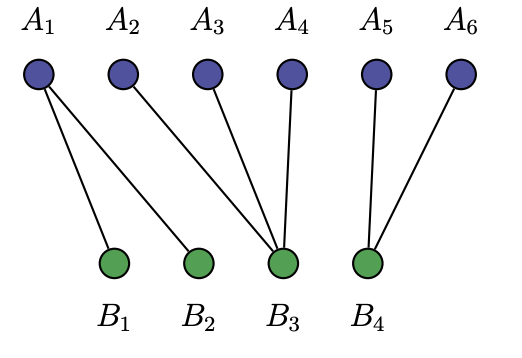
\includegraphics[scale=0.7]{a.png}
		\end{center}
		vec\_size[1] indica que tenemos 2 matches que salen de a.\\
		vec\_size[2] indica que tenemos 3 matches que salen de b.\\\\
		Como ya tenemos el match de cada fila de las matrices, podemos empezar con la animación. \\\\
		\textbf{Matriz intermedia}\\
		Generaremos una matriz intermedia entre A y B que se generará gracias al matching. 
		n. Si en el matching entre A[i] y B[i] hay una división, entonces es razonable que el bloque correspondiente en A[i] se divida en subloques proporcionales a los tamaños de los bloques correspondientes en B[i]. Por ejemplo, si un bloque, de tamaño 14 mediante una división termina en tres bloques de tamaño 10, 20, y 5. Entonces dicho bloque será dividido en subloques de 4, 8, 2, cada uno de los cuales ser irá transformando progresivamente en su correspondiente bloque en B[i].
		\\\\
		\underline{Aplicación}\\ 
		El paso final fue implementar una animación de transformación de imágenes, utilizando como parte inicial la captura de inputs diseñada en el ejercicio 8, y permitiendo el ingreso de un input que seleccione qué método de transformación utilizar. El resultado de la función implementada será transformado a una matriz binaria que representa la imagen resultado. Estas imágenes serán calculadas y guardadas dentro de un bucle, que permitirán su visualización.\\\\
		\begin{enumerate}
			\item 	Convertir el output de las transformaciones a binario.\\\\
			Esta función recibe como parámetro la transformación del output de las funciones implementadas anteriormente, y las interpreta hasta convertirla en una matriz binaria Answer. Para esto, usaremos una subrutina llamada Transformar, que recibe un matching de una de las filas de las imágenes y las interpreta y transforma a binario.\\
			\begin{algorithmic}[1]
				\TITLE{\textsc{MatchtoBin}$(image)$}
				\FOR {for i in m\_Match:}
				\STATE Answer[i] = Traducir(m\_Match, A[i], B[i]) 
				\ENDFOR
			\end{algorithmic}
		-\\
			En la función traducir es donde se empieza a crear la matriz intermedia. (Generándoce fila por fila de ambas matrices)
	\\\\
			Esta función lo que hace es agarrar los dos vectores A[i] y B[i]. Para generar el vector Mi[i] de la matriz intermedia.\\
			
		Por cada matching:\\
		011001000111 ----------------- 0001110000	
		
		Realiza la operación: $\lceil{x/y * n}\rceil$ 
		\\"cantidad de matches que tenga el bloque único" veces\\
		\\Donde:\\ x = peso de bloque único \\ y = peso de bloques al que se  conecta el bloque único \\ n = peso de cada bloque separado
		
		Y genera nuevo segmento de vector:
		
		010001000110				
		
		Cada nuevo peso de los bloques se almacenan en el vector que tenía los bloques divididos.
		
		\item Guardar la imagen como un archivo ppm insertando valores RGB.\\\\
		Posteriormente , a partir de la matriz Answer resultante de la función MatchtoBin, la podemos guardar como un texto de valores RGB y un formato .ppm utilizando la función WriteImage.\\
		
		\begin{algorithmic}[1]
			\TITLE{\textsc{WriteImage}$(Answer, archivo)$}
			\STATE archivo.write(info);
			\FOR {i in answer:}
			\STATE temp = encode(i) \#transforma una fila de binario a decimal.
			\STATE archivo.write(temp);
			\ENDFOR
		\end{algorithmic}
		\end{enumerate}
-\\Primera fila: Se aprecia la animación realizada con la transformación voraz.\\ Segunda fila: Animación con transformación dinámica.
		\begin{center}
			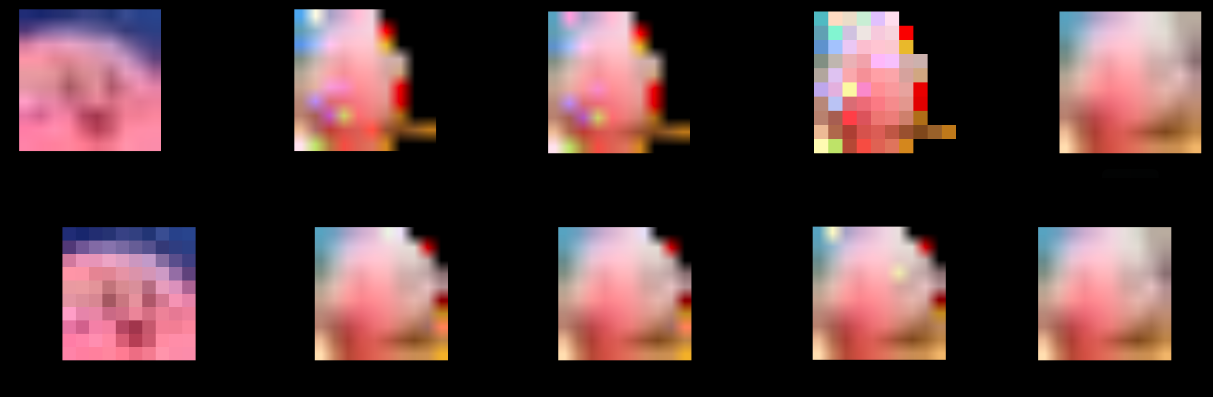
\includegraphics[scale=0.35]{b.png}
		\end{center}
		
		\subsection*{Pregunta 10 (Transformación Dinámica Mejorada)}
		Anteriormente con los algoritmos anteriores se buscaba maximizar B. Ahora con el uso de un nuevo algoritmo se podrá notar una curva más suave al momento de ejecutar la animación pporque se está buscando un equilibrio entre las dos imágenes\\\\
		Recibe:
		\begin{itemize}
			\item Matriz A y B
		\end{itemize}
		Devuelve: 
		\begin{itemize}
			\item Peso Promedio-transformación tipo Float
			\item Un matching por cada fila de la matriz
		\end{itemize}
		Aclaración
		\\
		\begin{algorithmic}
			\TITLE{\textsc{Transformación-Dinámica-Promedio}$(A, B)$}
		\end{algorithmic}
		-----------\\\\
		\textbf{Análisis de Tiempo}\\
		Misma complejidad de tiempo que la otra tranformación dinámica $T()=O(pq^2)$
		
\section{GitHub}
\href{https://github.com/mateonoel2/ProyectoADA}{https://github.com/mateonoel2/ProyectoADA}
\end{document}